\section{Veebirakenduse arhitektuur}
Kavandatava infosüsteemi komponendid:
\begin{itemize}
    \item \textbf{server} -- renditud pilverserver Ubuntu operatsioonisüsteemiga. Teenus kindlasti peab võimaldama operatsioonisüsteemi
    haldamist \textit{root}-rootkasutajana, et oleks võimalik Docker-i kaudu käivitada rakenduse serveriosa. Samuti süsteemis peab olema paigaldatud
    Apache veebiserver, mis serveerib veebirakenduse kasutajaliidese osa,
    \item \textbf{back-end} -- infosüsteemi serveriosa, käivitatud Docker-konteinerina serveri operatsioonisüsteemis,
    \item \textbf{front-end} -- serveri kasutajaliidese osa
    \item \textbf{andmebaas} -- andmete salvestamiseks, esialgselt paigaldatakse samale serverile.
\end{itemize}

\begin{figure}[ht]
    \centering
    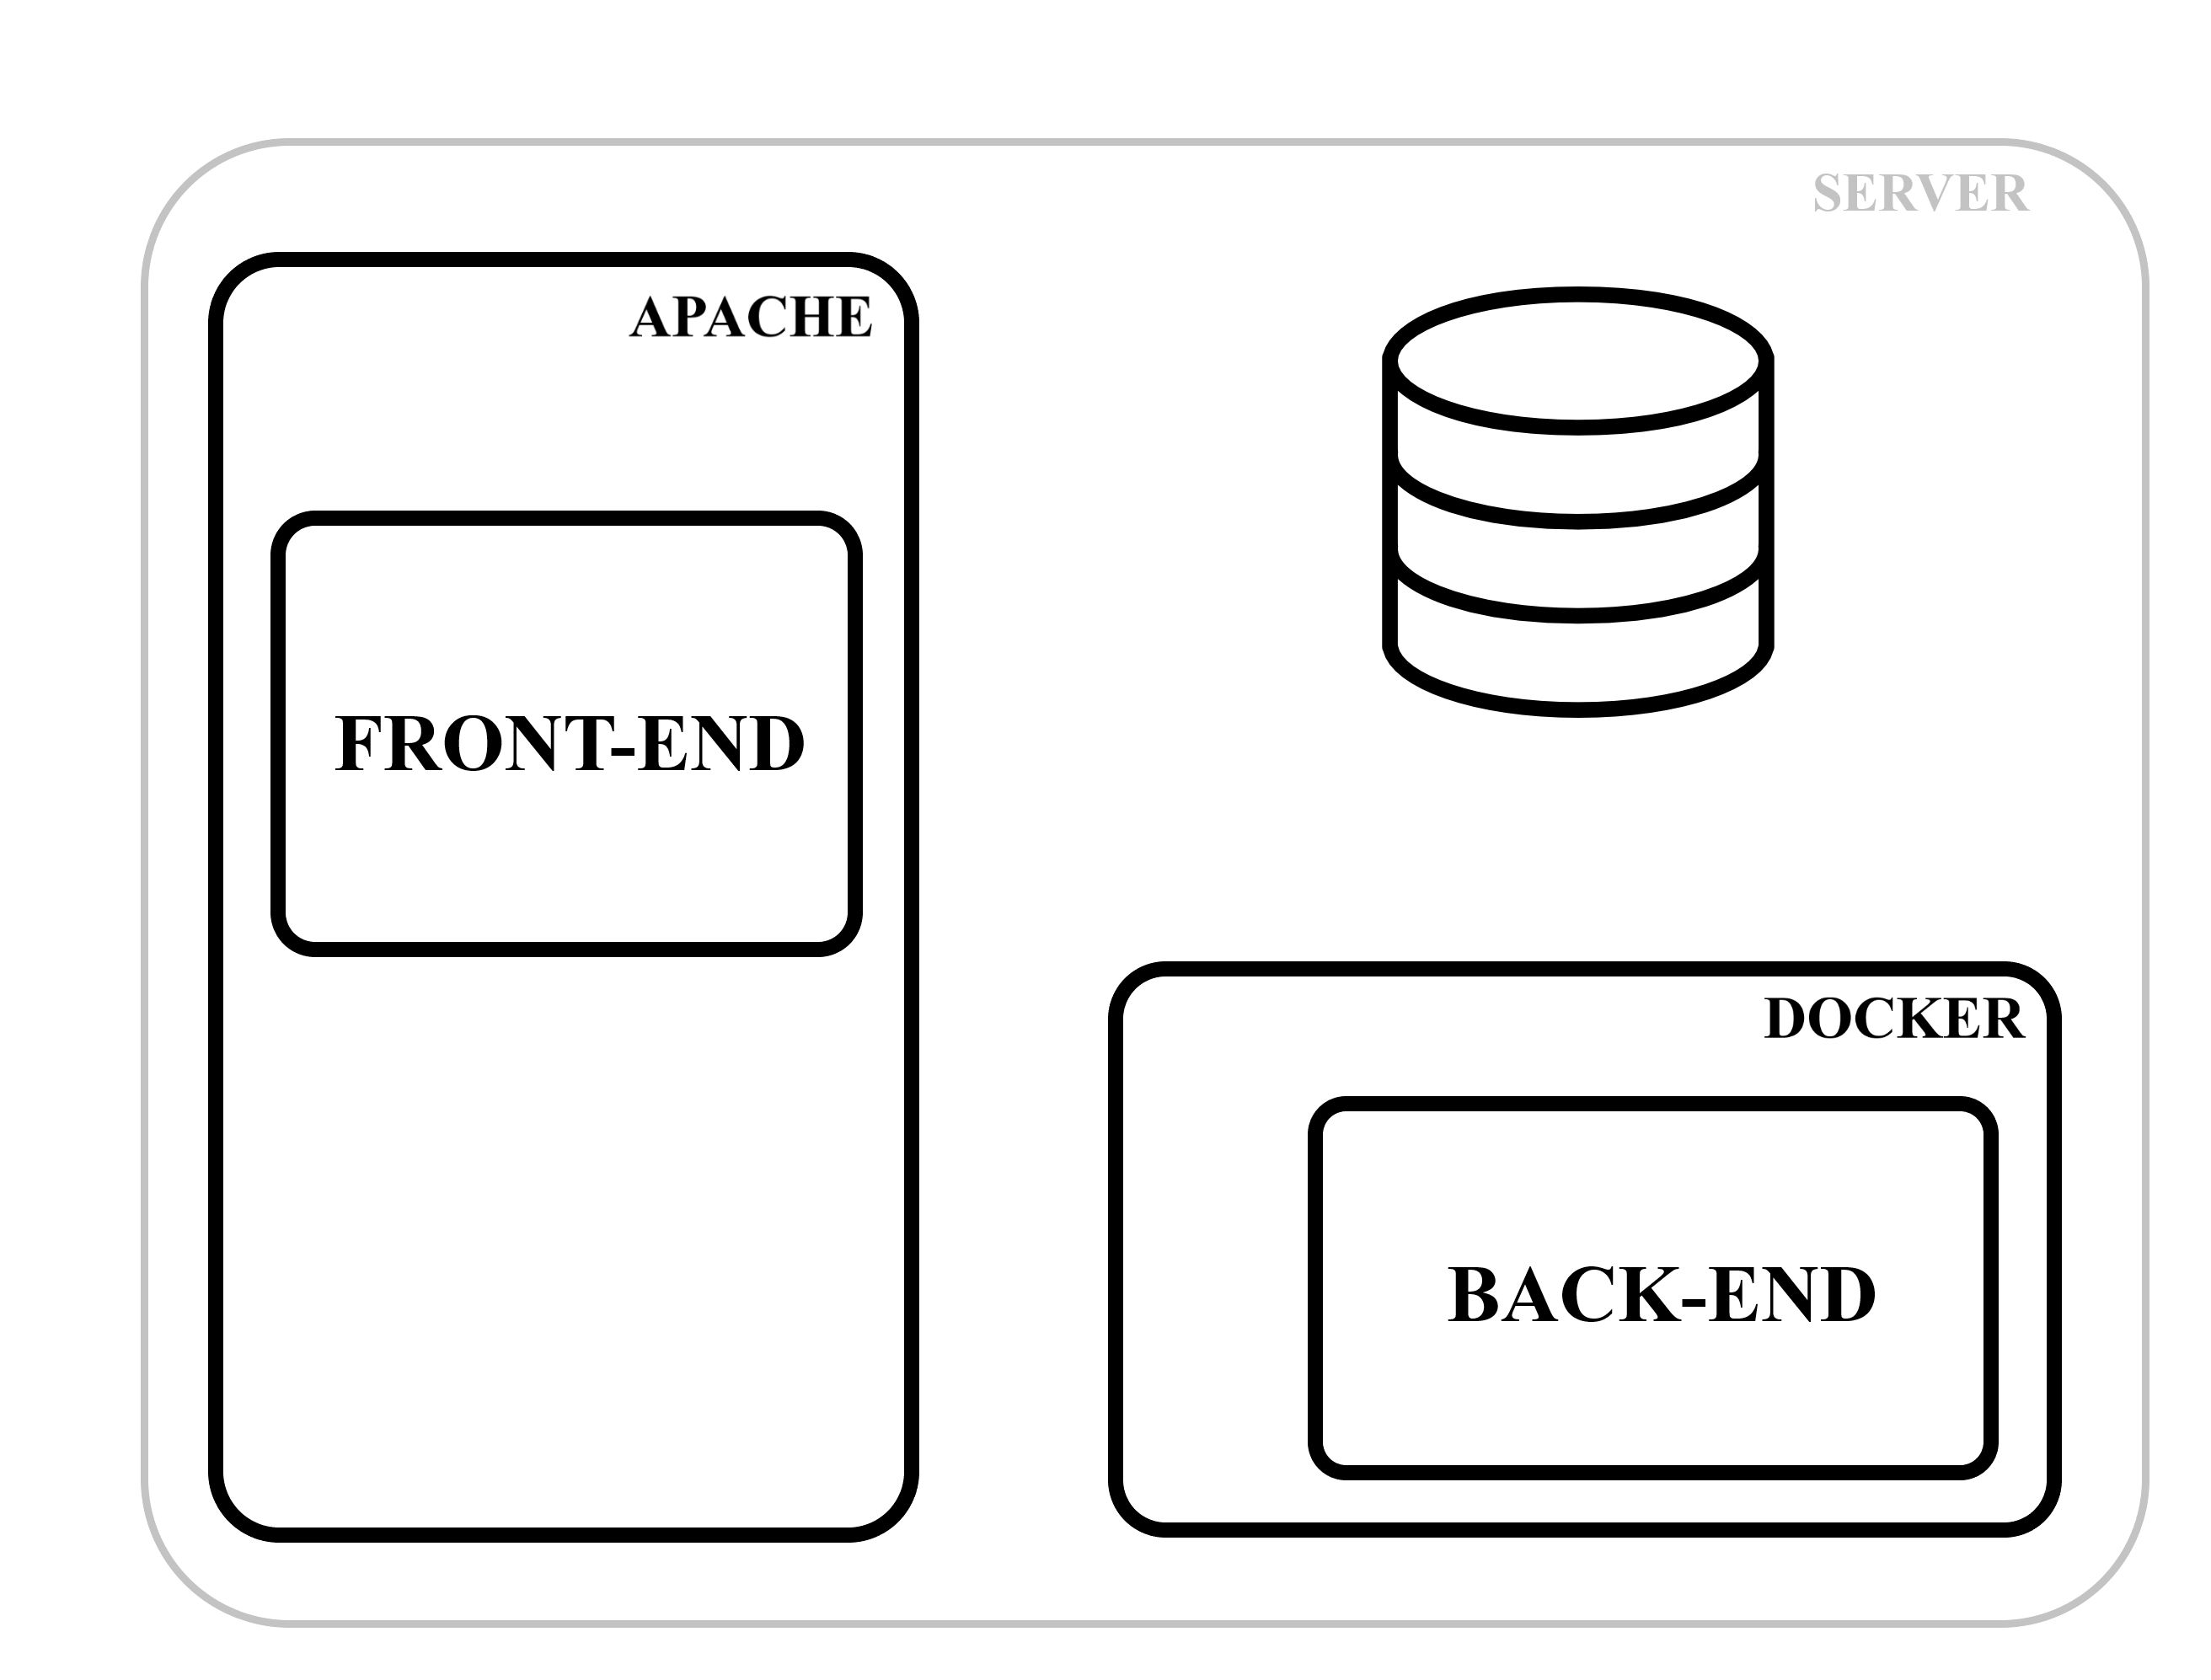
\includegraphics[width=0.6\textwidth]{figures/analysis/architecture.png}
    \caption[Infossüsteemi arhitektuur]{\textit{Infossüsteemi arhitektuur}}
    \label{fig:architecture}
\end{figure}